\usecolorstyle{TitleStyle}
\block[bodyinnersep=0em]{Perspectives }{}
\usecolorstyle{myColorStyle}

\begin{columns}

    \column{0.7}

    \block{\hspace{-600pt}Mesh adaptation}{
        \vspace{-20pt}
        \begin{center}
            \begin{minipage}{0.6\linewidth}
                \begin{tcolorbox}[
                    colback=color1!50, % Couleur de fond de la boîte
                    colframe=color2, % Couleur du cadre de la boîte
                    arc=2mm, % Rayon de l'arrondi des coins
                    boxrule=2pt, % Épaisseur du cadre de la boîte
                    breakable, enhanced jigsaw,
                    width=\linewidth
                    ]       
                    \textbf{Construction of the mesh:} $N_\text{dofs}=598$.

                    \begin{minipage}{0.48\linewidth}  
                        \centering\vspace{10pt}
                        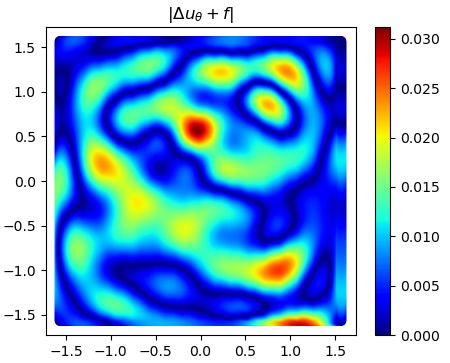
\includegraphics[width=\linewidth]{images/persp/residual_test1_v1_param1_mesh1.png}
                    \end{minipage} \;
                    \begin{minipage}{0.48\linewidth} 
                        \flushright\vspace{-20pt}
                        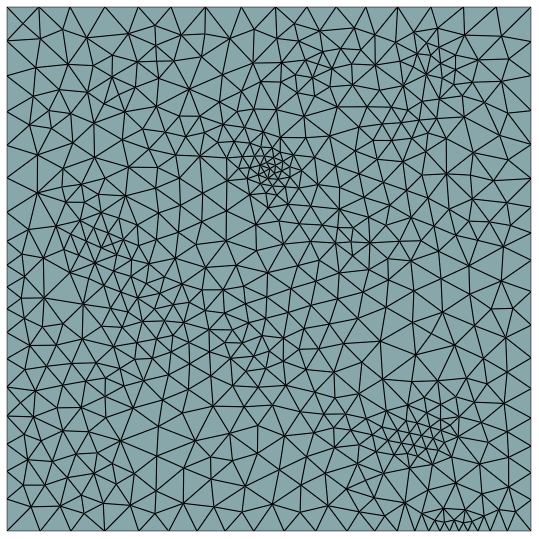
\includegraphics[width=0.85\linewidth]{images/persp/Mesh_plot_case1_v1_meshfromnet1.png}
                    \end{minipage}
                \end{tcolorbox}
            \end{minipage}
            \begin{minipage}{0.38\linewidth}
                \vspace{-70pt}
                \begin{tcolorbox}[
                    colback=color1!50, % Couleur de fond de la boîte
                    colframe=color2, % Couleur du cadre de la boîte
                    arc=2mm, % Rayon de l'arrondi des coins
                    boxrule=2pt, % Épaisseur du cadre de la boîte
                    breakable, enhanced jigsaw,
                    ]       
                    \textbf{Apply enriched FEM:}

                    \hspace{-40pt}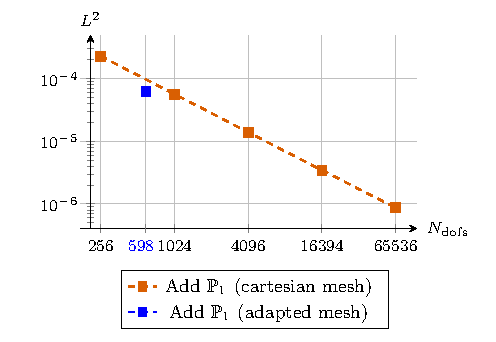
\includegraphics[width=1.1\linewidth]{images/numeric/poisson/dirichlet/persp/persp.pdf}
                \end{tcolorbox}
            \end{minipage}
        \end{center}
        \vspace{-30pt}
    }

    \usecolorstyle{bibStyle}
    \useblockstyle{Default}
	\block{
		\vspace{-40pt}
        \AtNextBibliography{\normalsize}
		\printbibliography[heading=none]
	}

    \column{0.3}

    \usecolorstyle{myColorStyle}
    \useblockstyle{TornOut}

    % \block{Complex geometry}{
    %     \vspace{-20pt}
    %     \begin{center}
    %         \vspace{-20pt}
    %         \hspace{200pt}
\includegraphics[width=0.58\linewidth]{images/persp/cat.png}
            
    %         \vspace{-100pt}
    %         \hspace{-220pt}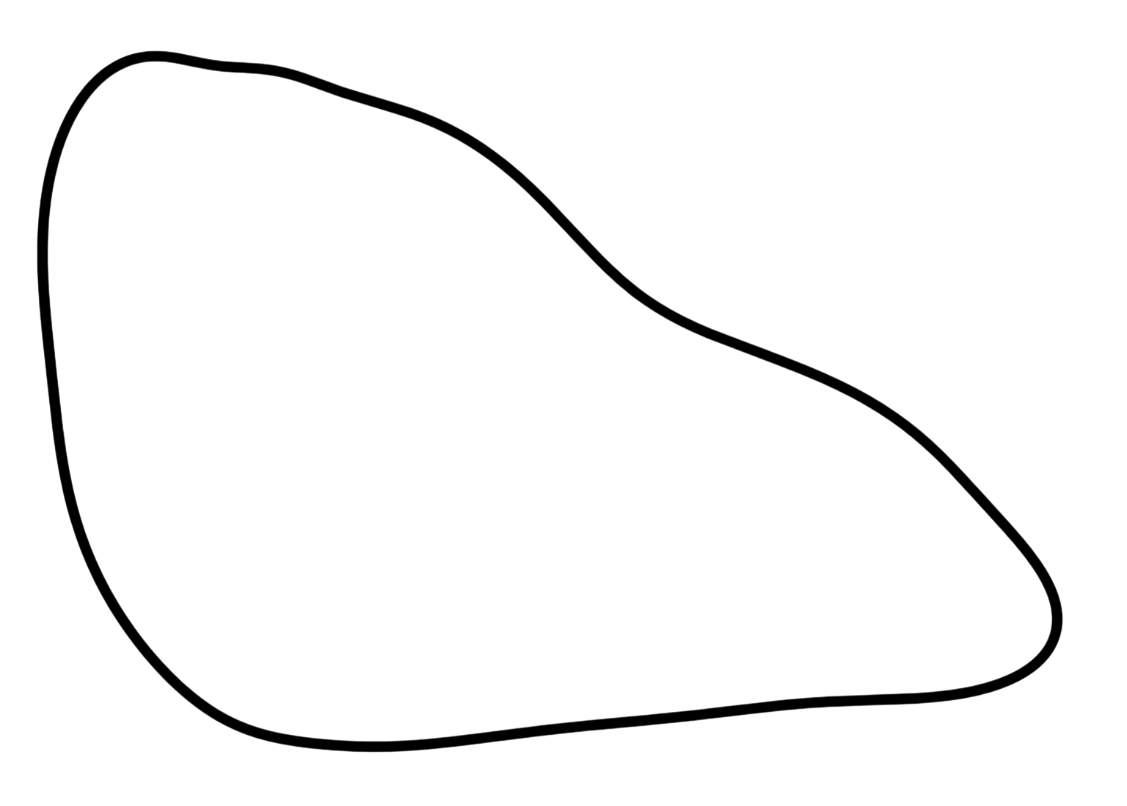
\includegraphics[width=0.6\linewidth]{images/persp/liver.png}
    %     \end{center}
    %     \vspace{-30pt}
    % }

    \block{Complex geometries}{
        % \vspace{-20pt}
        \begin{center}
            \vspace{-20pt}
            \flushright
\includegraphics[width=0.68\linewidth]{images/persp/cat.png}
            
            \vspace{-80pt}
            \flushleft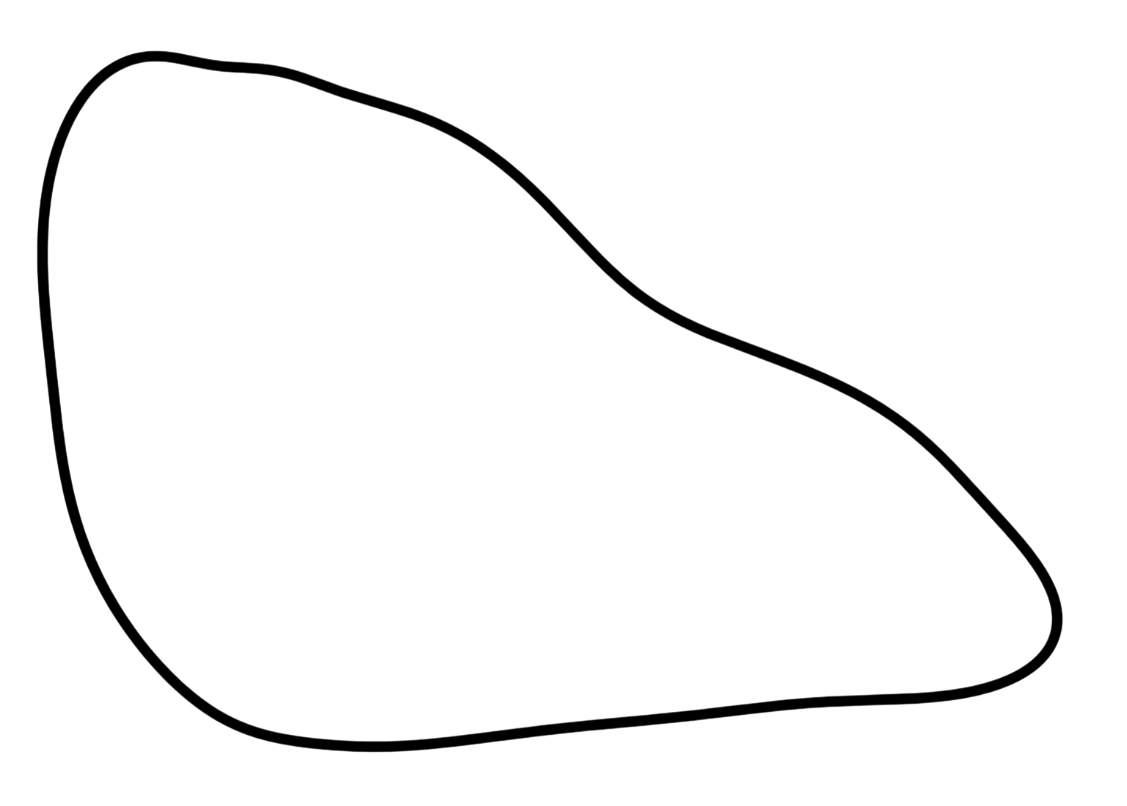
\includegraphics[width=0.7\linewidth]{images/persp/liver.png}
        \end{center}
        \vspace{-30pt}
    }


\end{columns}